\documentclass[10pt]{article}

\usepackage{fullpage}
\usepackage{setspace}
\usepackage{parskip}
\usepackage{titlesec}
\usepackage[section]{placeins}
\usepackage{xcolor}
\usepackage{breakcites}
\usepackage{lineno}
\usepackage{hyphenat}

\setlength\columnsep{25pt}





\PassOptionsToPackage{hyphens}{url}
\usepackage[colorlinks = true,
            linkcolor = blue,
            urlcolor  = blue,
            citecolor = blue,
            anchorcolor = blue]{hyperref}
\usepackage{etoolbox}
\makeatletter
% \patchcmd\@combinedblfloats{\box\@outputbox}{\unvbox\@outputbox}{}{%
%   \errmessage{\noexpand\@combinedblfloats could not be patched}%
% }%
\makeatother


\usepackage{natbib}




\renewenvironment{abstract}
  {{\bfseries\noindent{\abstractname}\par\nobreak}\footnotesize}
  {\bigskip}

\titlespacing{\section}{0pt}{*3}{*1}
\titlespacing{\subsection}{0pt}{*2}{*0.5}
\titlespacing{\subsubsection}{0pt}{*1.5}{0pt}


\usepackage{authblk}


\usepackage{graphicx}
\usepackage[space]{grffile}
\usepackage{latexsym}
\usepackage{textcomp}
\usepackage{longtable}
\usepackage{tabulary}
\usepackage{booktabs,array,multirow}
\usepackage{amsfonts,amsmath,amssymb}
\providecommand\citet{\cite}
\providecommand\citep{\cite}
\providecommand\citealt{\cite}
% You can conditionalize code for latexml or normal latex using this.
\newif\iflatexml\latexmlfalse
\providecommand{\tightlist}{\setlength{\itemsep}{0pt}\setlength{\parskip}{0pt}}%

\AtBeginDocument{\DeclareGraphicsExtensions{.pdf,.PDF,.eps,.EPS,.png,.PNG,.tif,.TIF,.jpg,.JPG,.jpeg,.JPEG}}

\usepackage[utf8]{inputenc}
\usepackage[ngerman,greek,english]{babel}



\usepackage{float}






% Edit this header.tex file to include frontmatter definitions and global macros

% Add here any LaTeX packages you would like to load in all document blocks
% \usepackage{xspace}

% Add here any LaTeX macros you would like to load in all document blocks
% \def\example{This is an example macro.}

% -----

\iflatexml
% Add here any LaTeXML-specific commands

% -----

\else
% Add here any export style-specific LaTeX commands. These will only be loaded upon document export. 
% \paperfield{Subject domain of my document}
% \keywords{keyword1, keyword2}
% \corraddress{Author One PhD, Department, Institution, City, State or Province, Postal Code, Country}
% \fundinginfo{Funder One, Funder One Department, Grant/Award Number: 123456.}
\fi


\begin{document}

\title{The Ultraviolet Environment of a Tropical Megacity in Transition: Mexico
City 2000-2019}


\author[1,2]{Adriana Ipiña}
\author[3]{Gamaliel López-Padilla}
\author[4]{Armando Retama}
\author[1]{Rubén D. Piacentini}
\author[5]{Sasha Madronich}

\affil[1]{Instituto de Física Rosario (CONICET-UNR), Rosario, Argentina}
\affil[2]{Centro de Ciencias de la Atmósfera, Universidad Nacional Autónoma de México, Mexico City, Mexico}
\affil[3]{Facultad de Ciencias Físico Matemáticas, Universidad Autónoma de Nuevo León, San Nicolás de los Garza, México}
\affil[4]{Independent researcher, Mexico City, Mexico}
\affil[5]{National Center for Atmospheric Research, Boulder, Colorado, USA}


\vspace{-1em}



  \date{}


\begingroup
\let\center\flushleft
\let\endcenter\endflushleft
\maketitle
\endgroup


\linenumbers



\doublespacing


\selectlanguage{english}
\begin{abstract}
Tropical regions experience naturally high levels of UV radiation, but
urban pollution can reduce these levels substantially. We analyzed 20
years of measurements of the UV Index (UVI) at several ground-level
locations in the Mexico City Metropolitan Area and compared these with
UVI values estimated from satellite overpasses observing ozone and
clouds (but not local pollution). The ground-based measurements were
systematically lower than the satellite-based estimates, by ca. 40\% in
2000 and 30\% in 2019. Calculations with a radiative transfer model and
observed concentrations of air pollutants explained well the difference
between satellite- and ground-based UVI, and showed specific
contributions from boundary layer aerosols, O\textsubscript{3},
NO\textsubscript{2}, and SO\textsubscript{2}, in decreasing order of
importance. Such large changes in UV radiation have important
implications ranging from human health (skin cancer and cataract
induction) to air pollution control (photochemical smog formation).%
\end{abstract}%



\sloppy


Keywords: Ultraviolet radiation, UV~Index, Megacities, Air pollution,
Urban photochemistry.

Synopsis: Improvements in Mexico City's air quality during 2000-2019
were accompanied by increases in UV radiation, augmenting human exposure
and photochemical smog formation.

\section*{Introduction}

{\label{123750}}

Ultraviolet (UV) radiation is an important component of the urban
environment, affecting human populations directly through UV exposure of
skin and eyes\textsuperscript{\hyperref[csl:1]{1},\hyperref[csl:2]{2},\hyperref[csl:3]{3}} and less directly (but with great
impact) by driving the formation of photochemical smog, including
tropospheric ozone and other oxidants, as well as secondary aerosols
containing nitrates, sulfates, and organics.\textsuperscript{\hyperref[csl:4]{4},\hyperref[csl:5]{5},\hyperref[csl:6]{6}} These
pollutants, along with others of primary origin commonly found in urban
atmospheres (e.g., black carbon, sulfur dioxide), can in turn scatter
and/or absorb UV radiation, alter its vertical distribution, and so
modify the photochemical rate of their own formation. Such feedback
complicates the calculation of both the UV radiation field (including at
the surface), and the evolution of photochemical smog in the urban
boundary layer.

The question of how air pollution alters the urban UV environment
(and~\emph{vice versa}) is not new, but studies have relied mostly on
numerical models,\textsuperscript{\hyperref[csl:7]{7},\hyperref[csl:8]{8},\hyperref[csl:9]{9}} with relatively fewer available
observations (e.g.,~\emph{McKenzie et
al.\textsuperscript{\hyperref[csl:10]{10}}};~\emph{Panicker et
al.}\textsuperscript{\hyperref[csl:11]{11}};~\emph{Palancar et al}.\textsuperscript{\hyperref[csl:12]{12}};
reviewed by Bais et al.\textsuperscript{\hyperref[csl:13]{13}}). Increases in UV have been
estimated in association with decadal emission reductions, e.g. in
China,\textsuperscript{\hyperref[csl:14]{14},\hyperref[csl:15]{15},\hyperref[csl:16]{16}} and have led to less-than-expected reductions
in photochemical smog, in part due to stronger UV
photochemistry.\textsuperscript{\hyperref[csl:17]{17},\hyperref[csl:18]{18},\hyperref[csl:19]{19}} Emission reductions have also occurred
globally during the 2020 COVID-19 pandemic,\textsuperscript{\hyperref[csl:20]{20},\hyperref[csl:21]{21}} but
ground-level ozone in polluted have actually
increased,\textsuperscript{\hyperref[csl:22]{22},\hyperref[csl:23]{23}} due at least in part to the increased UV
radiation. Unfortunately, the observational data base of relevant UV
radiation remains rather sparse to evaluate such model-derived
hypotheses.~~

The environment of Mexico City is of particular interest for several
reasons: (1) Nearly 23 million people inhabit the Mexico City
Metropolitan Area (MCMA), and the UV environment has direct implications
for their health, both in terms of skin/eye UV exposure and~\emph{via}
photochemical smog formation. (2) As a tropical megacity, it is to some
extent representative of the situation of many others, with year-round
intense midday UV irradiance, a shallower atmosphere due to significant
elevation above sea level, and a transition toward newer and cleaner
technologies, leading to gradual improvements in air quality. (3) Air
quality within MCMA has undergone extensive scrutiny, with
well-established monitoring network since 1986,\textsuperscript{\hyperref[csl:24]{24}}
numerous intensive field campaigns to study the meteorology, emissions,
and photochemistry of smog formation,\textsuperscript{\hyperref[csl:25]{25},\hyperref[csl:26]{26},\hyperref[csl:27]{27}} and numerical
modeling incorporating the evolving knowledge.\textsuperscript{\hyperref[csl:28]{28},\hyperref[csl:29]{29},\hyperref[csl:30]{30},\hyperref[csl:31]{31}} This
extensive body of knowledge provides the foundation for understanding
our study.

Here, we analyze two decades of continuous measurements of the UV Index
at multiple locations within the MCMA, collected by the Secretariat of
the Environment (Secretar\selectlanguage{ngerman}ía del Medio Ambiente, SEDEMA) of the Mexico
City government as part of an intensive monitoring network over the
MCMA.\textsuperscript{\hyperref[csl:32]{32}}~The UV Index is defined as:

\begin{equation}
\label{eq:UVI}
UVI=40 \int_{250nm}^{400nm} E\left(\lambda,t\right) \cdot S_{er}(\lambda) d\lambda
\end{equation}

where~\(E(\lambda,t)\)\emph{~} is the solar spectral irradiance in
units of W/(m\textsuperscript{2} ·nm) and~\(S_{er}\left(\lambda\right)\) is the
erythemal sensitivity of human skin.\textsuperscript{\hyperref[csl:33]{33},\hyperref[csl:34]{34}} Multiplication by
40 is chosen historically to yield small integer scales, but is
otherwise scientifically arbitrary.

The UVI is recognized by the World Health and Meteorological
Organizations (WHO and WMO) as a standardized metric of UV
radiation\textsuperscript{\hyperref[csl:33]{33}} for global public information. An advantage
of using the UVI as (one) metric of UV radiation is that it is being
increasingly observed or calculated and disseminated, enabling more
objective comparisons between seasons and locations. The UVI
observations from Mexico City, considered here, are an important element
of this global picture. ~

While the UVI at the surface cannot be translated directly into
photolysis frequencies for various photo-labile molecules, the spectral
weighting of the UVI (ca. 300-320 nm) is approximately similar to that
for the photolysis of ozone to singlet oxygen atoms. Other UV
wavelengths are of course also important, e.g. for the photolysis of
nitrogen dioxide, and may be affected differently depending on the
pollutant. With these considerations and a few other \emph{caveats}, UVI
trends examined here can also be used to infer accompanying trends in
photolysis frequencies.

\section*{Methods}

{\label{770133}}

\subsection*{Ground-based measurements}

{\label{220276}}

The Mexico City Metropolitan Area is located at 19.4°N, 99.1°W, 2240
meters above sea level (asl), surrounded by mountain ridges exceeding
5000 m asl, with complex topography and thermal inversions that inhibit
winds and favor intense air pollution.\textsuperscript{\hyperref[csl:35]{35},\hyperref[csl:36]{36}} Air quality
monitoring and surface meteorological measurements in the MCMA are
conducted~continuously by the Atmospheric Monitoring System (SIMAT, by
its Spanish acronym) of the Mexico City Government. Since the year 2000,
UV radiometers (model 501-A, Solar Light Company Inc., Glenside, PA)
detecting wavelengths between 280-400 nm have been measuring
erythemally-weighted solar radiation. The calibrations were carried out
annually, using a periodically calibrated reference sensor from the same
manufacturer. Although at the beginning only a few stations were in
operation and have been changing, currently 11 stations are recording
erythemal irradiances, which are then multiplied by 40 (see
Eq.~{\ref{eq:UVI}}) to give UV Indices.
Table~{\ref{table:stations}} describes the location of
the stations where UV Index has been measured.
Figure~{\ref{977905}} shown the radiometers of the
SIMAT have been distributed over MCMA, prioritizing the sites with more
density of population. Near real-time data for each station are
available on the SIMAT official
website~\url{http://www.aire.cdmx.gob.mx/default.php}.\selectlanguage{english}
\begin{table}[H]
\centering 
\begin{tabular}{ccccc}
\hline
Station&Environment &Lat (\selectlanguage{ngerman}°N) &Lon (\selectlanguage{ngerman}°W)&El (masl)\\ \hline
CHO &school zone&19.27&99.89&2253\\ 
CUT &ecological park&19.72&99.20&2263\\
FAC &urban&19.48&99.24&2299\\
HAN &urban&19.42&99.08&2235\\
LAA &urban&19.48&99.15&2255\\
MER&downtown&19.42&99.12&2245\\
MON&rural&19.46&98.90&2252\\
MPA&rural&19.18&98.99&2594\\
PED&residential &19.33&99.20&2326\\
SAG&urban&19.53&99.03&2241\\
SFE&residential &19.36&99.26&2599\\
TLA&urban &19.53&99.20&2311\\ 
CCA &University city&  19.33 & 99.18 & 2294\\\hline
\end{tabular}
\caption{\selectlanguage{ngerman}{{{SIMAT stations, environmental descriptors and geographical positions. Abbreviations names: Chalco (CHA), Cuautitlán (CUT), FES Acatlán (FAC), Hangares (HAN), Laboratorio de Análisis Ambiental (LAA), Merced (MER), Montecillo (MON), Milpa Alta (MPA), Pedregal (PED), San Agustín (SAG), Santa Fe (SFE), Centro de Ciencias de la Atmósfera (CCA) and Tlalnepantla (TLA). }}}}
\label{table:stations}
\end{table}\selectlanguage{ngerman}\selectlanguage{english}
\begin{figure}[H]
\begin{center}
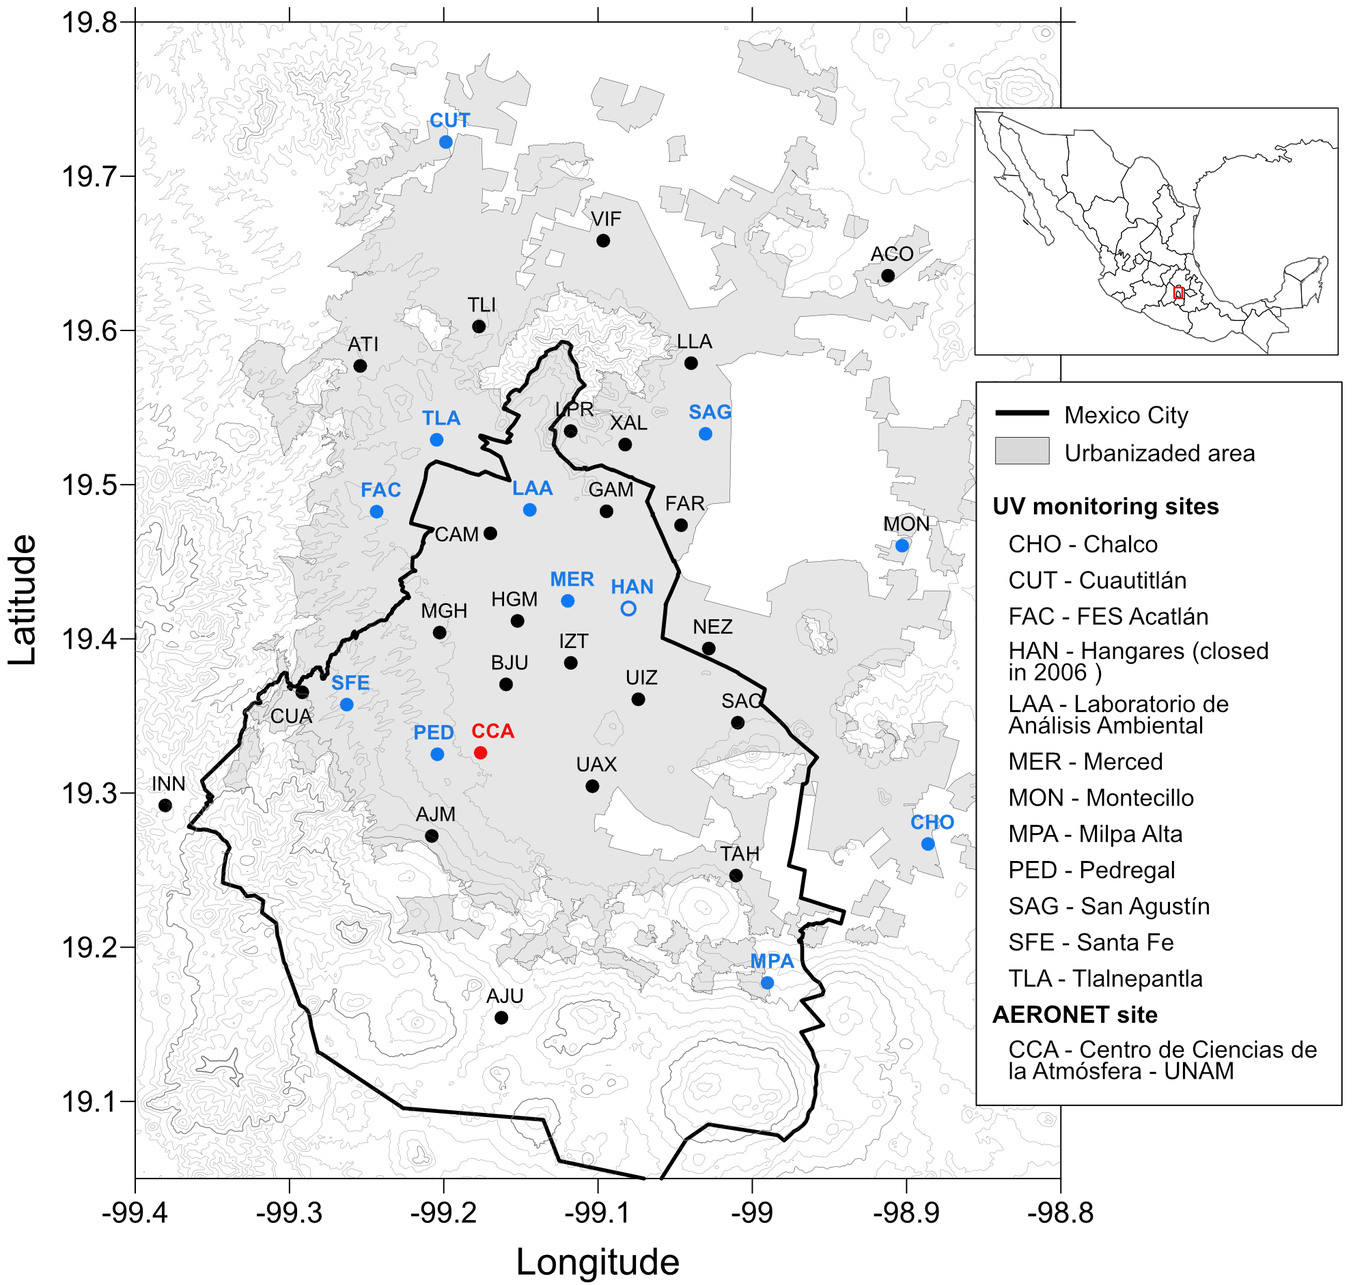
\includegraphics[width=0.70\columnwidth]{figures/MapaUV v4Dec20/MapaUV v4Dec20}
\caption{{Map with the location of the SIMAT continuos monitoring stations over
MCMA. Sites denoted by the blue solid dots correspond to the sites were
UV had been measured, the site on open blue dot denoted a discontinued
site, the red dot corresponds to the location of the AERONET site. The
location~of Mexico City and the acronyms of the UV and AERONET site are
shown at the upper and lower frames at the rigth, respectively.
{\label{977905}}%
}}
\end{center}
\end{figure}

With the aim to explore the relationship between UVI and air pollutants
levels, the hourly averages for ozone (O\textsubscript{3}), carbon
monoxide (CO), nitrogen dioxide (NO\textsubscript{2}), sulfur
dioxide~(SO\textsubscript{2}) and particle matter with diameter
sizes~\(\le\) 10 micrometers (PM\textsubscript{10}), were
downloaded from the SIMAT\textsuperscript{\hyperref[csl:37]{37}}. Only values obtained
between 11h and 14h CST were considered for the trends analysis.
Pollutants measurements are conducted by the SIMAT using
regulatory-grade commercial instruments. Measurement principles include
ultraviolet photometry (model 400E, Teledyne-API) for
O\textsubscript{3}, chemiluminescence (model 200E, Teledyne-API) for
NO\textsubscript{2}, UV fluorescence (model 100E, Teledyne API) for
SO\textsubscript{2}, and infrared absorption (model 300E, Teledyne-API)
for CO. The PM\textsubscript{10} continuous mass concentration was
measured with Tapered Element Oscillating Microbalance (TEOM 1400AB or
TEOM 1405 DF, Thermo Scientific) monitors. Gaseous pollutant levels are
reported in ppb concentration units for O\textsubscript{3},
SO\textsubscript{2} and NO\textsubscript{2}, and in ppm for CO.
Particulate matter mass concentration is reported in \selectlanguage{greek}µ\selectlanguage{english}g
m\textsuperscript{-3} at local conditions for temperature and pressure.

Aerosol optical depth at 340 nm was obtained from the Centro de Ciencias
de la Atm\selectlanguage{ngerman}ósfera (CCA), measurements were conducted with a photometer of
the AErosol RObotic NETwork (AERONET\textsuperscript{\hyperref[csl:38]{38}}). The data
Product Level 2.0 were selected, and annual averages
AOD\textsubscript{340} were calculated from continuous measurements
during at least 7 months\textsubscript{.}

\subsection*{Satellite data}

{\label{800866}}

Estimates of the UV Index from satellite-based measurements of clouds
and O\textsubscript{3} were used for comparing to the ground-based
measurements. These data were provided by the Ozone Monitoring
Instrument (OMI)~on board of AURA-NASA satellite.\textsuperscript{\hyperref[csl:39]{39}} OMI
was created in cooperation between the Netherlands Agency for Aerospace
Programmes (NIVR), the Finnish Meteorological Institute (FMI) and NASA.
OMI (hereafter OMI-Aura/NIVR-FMI-NASA) performs observations over a
geographical dimension of 13 × 24km\textsuperscript{2} at nadir. For
Mexico City, the satellite overpass time is between 19:00h - 21:00h UTC
and data are specific for the coordinates and elevation of Mexico City.
To our knowledge, no correction is made for local air pollution.

\subsection*{TUV model}

{\label{308972}}

Calculations of the UV Index were also made with the Tropospheric
Ultraviolet Visible (TUV v5.3) model.\textsuperscript{\hyperref[csl:40]{40}} The model
vertical structure was modified to place the surface at 2.24 km asl,
overlain by a 3 km boundary layer\textsuperscript{\hyperref[csl:41]{41},\hyperref[csl:36]{36}} in which the aerosol
optical depth (AOD) and the concentrations of gaseous
O\textsubscript{3}, NO\textsubscript{2}, and SO\textsubscript{2} can be
varied. Above the atmospheric boundary layer (ABL) (i.e. above 5.24 km
asl) the model defaults to a climatological continental aerosol
profile\textsuperscript{\hyperref[csl:42]{42}} whose remaining optical depth (i.e. from 5.24
km to space) is 0.23 at 340 nm, and O\textsubscript{3} profile from the
US Standard Atmosphere with the total ozone column scaled to a
climatological value of 265 Dobson Units. ABL aerosols are modeled by
prescribing the AOD at 340 nm (from AERONET observations), scaled to
other wavelengths inversely with wavelength (Angstrom coefficient =
1.0), asymmetry factor of 0.7, and a single scattering albedo of 0.85 at
UV wavelengths, following the determinations made in Mexico City by Corr
et al.\textsuperscript{\hyperref[csl:43]{43}} and Palancar et al.\textsuperscript{\hyperref[csl:12]{12}}.
Radiative transfer calculations were carried out with the
pseudo-spherical 4-stream option.

\section*{Results and Discussion}

{\label{447962}}

Figure~{\ref{628947}} shows the diurnal variation of
the UVI for several specific cloud-free days, for different seasons and
several locations. Peak values range from 8 during autumn/winter to
almost 12 in spring/summer, in correspondence to the respective December
and June solstices, and follow closely the yearly variation of the
cosine of the solar zenith angle at noon (see
Figure~{\ref{310112}}). Although the stations are all
within a 25 km radius, substantial differences among them are notable.
The differences are particularly evident in the afternoons,~when air
pollutants have significantly accumulated within the boundary layer and
the mixing height is maximum, suggesting that their origin is not
related to calibration biases between the instruments. Survey of the
locations revealed that shadowing from nearby structures is not an
issue. It is more likely that local differences in air pollution,
particularly aerosols, are the cause of this variability. Previous
studies~(e.g., Castro et al.\textsuperscript{\hyperref[csl:44]{44}}~and Palancar et
al.\textsuperscript{\hyperref[csl:12]{12}})~have shown that surface UV radiation in Mexico
City is attenuated significantly by aerosols. The measurements shown in
Fig~{\ref{628947}} are consistent with increasing
pollution during the course of the day, with highest aerosol loading
(and highest variability) attained in the afternoon. Further support for
the role of pollution in suppressing the UVI comes from the observation
made at Santa Fe (SFE) site which in
Fig.~{\ref{628947}} are seen to be systematically
higher, e.g. by over 10\% in autumn afternoons, compared to the other
stations. The SFE station is located at 2600 m asl, approximately 300 m
higher than Mexico City downtown, and so avoids a substantial fraction
of the polluted MCMA boundary layer.\textsuperscript{\hyperref[csl:45]{45}} It is indeed
expected to have higher values of the UVI, in agreement with the
observations.\selectlanguage{english}
\begin{figure}[H]
\begin{center}
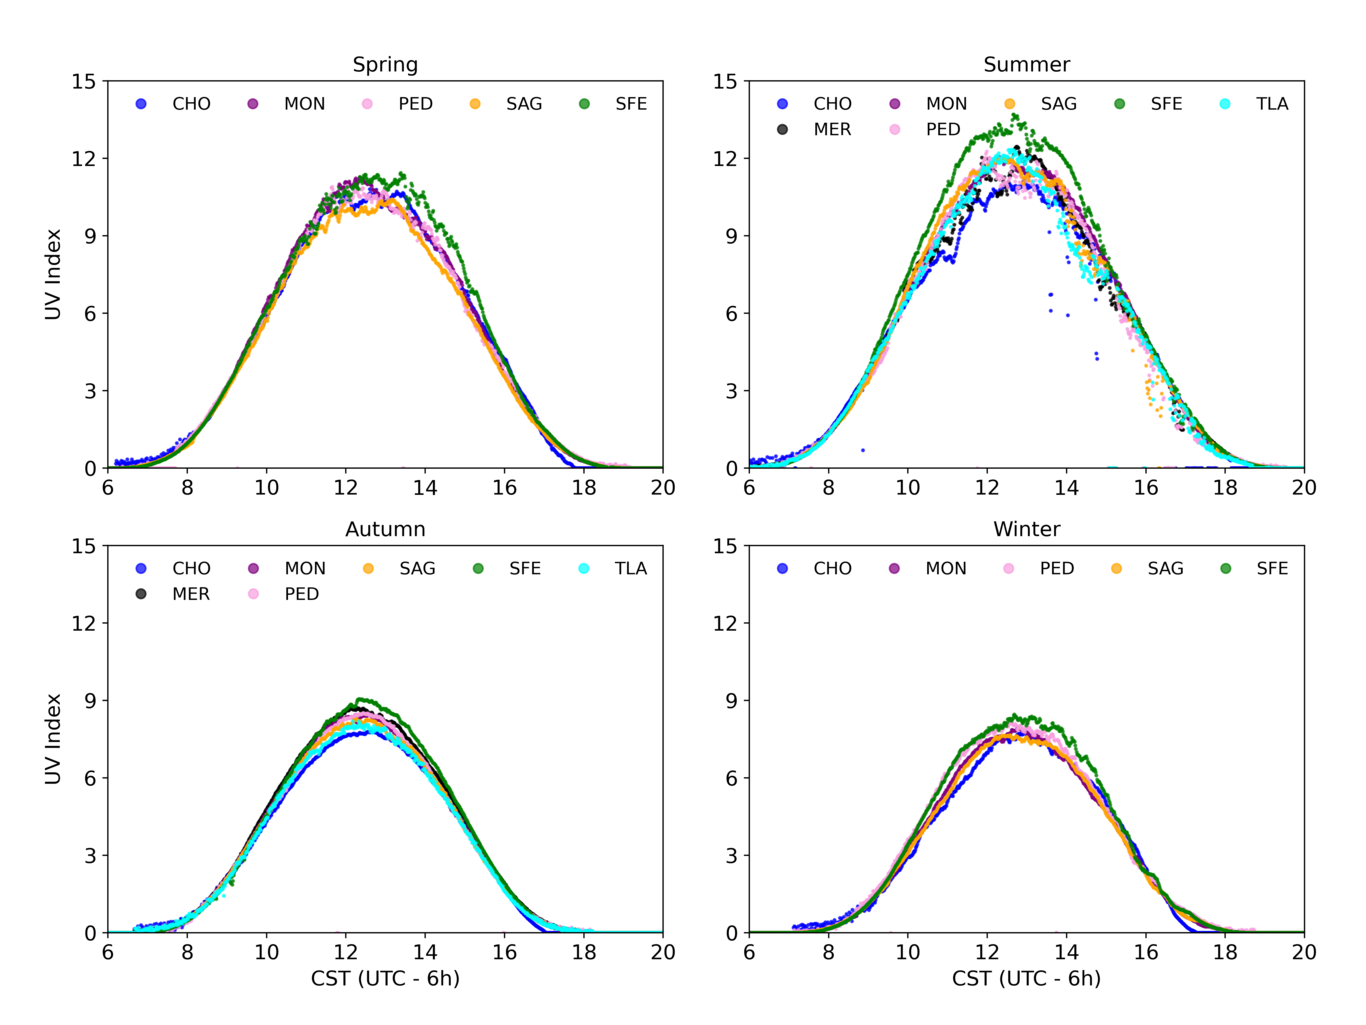
\includegraphics[width=0.70\columnwidth]{figures/season/season}
\caption{{UV Index measured over MCMA by SIMAT stations each minute along the day
under cloudless conditions for the seasons and dates (month/day/year):
Spring (04/20/2018), Summer (06/23/2018), Autumn (11/13/2018) and Winter
(02/02/2018).
{\label{628947}}%
}}
\end{center}
\end{figure}

Daily maximum values,~\(UVI_{\max}\), were extracted from the time
interval 11:00 h-14:00 h CST from each of the stations, with 7305
continuous days of measurements, during the period 2000-2019. As shown
in Figure~{\ref{461017}}, these values ranged from 1 to
15, with a majority (62\%) of the days experienced~\(UVI_{\max}\)
values between 6 and 10, and remarkably few, less than 1\%, in the
higher 13-15 range.\selectlanguage{english}
\begin{figure}[H]
\begin{center}
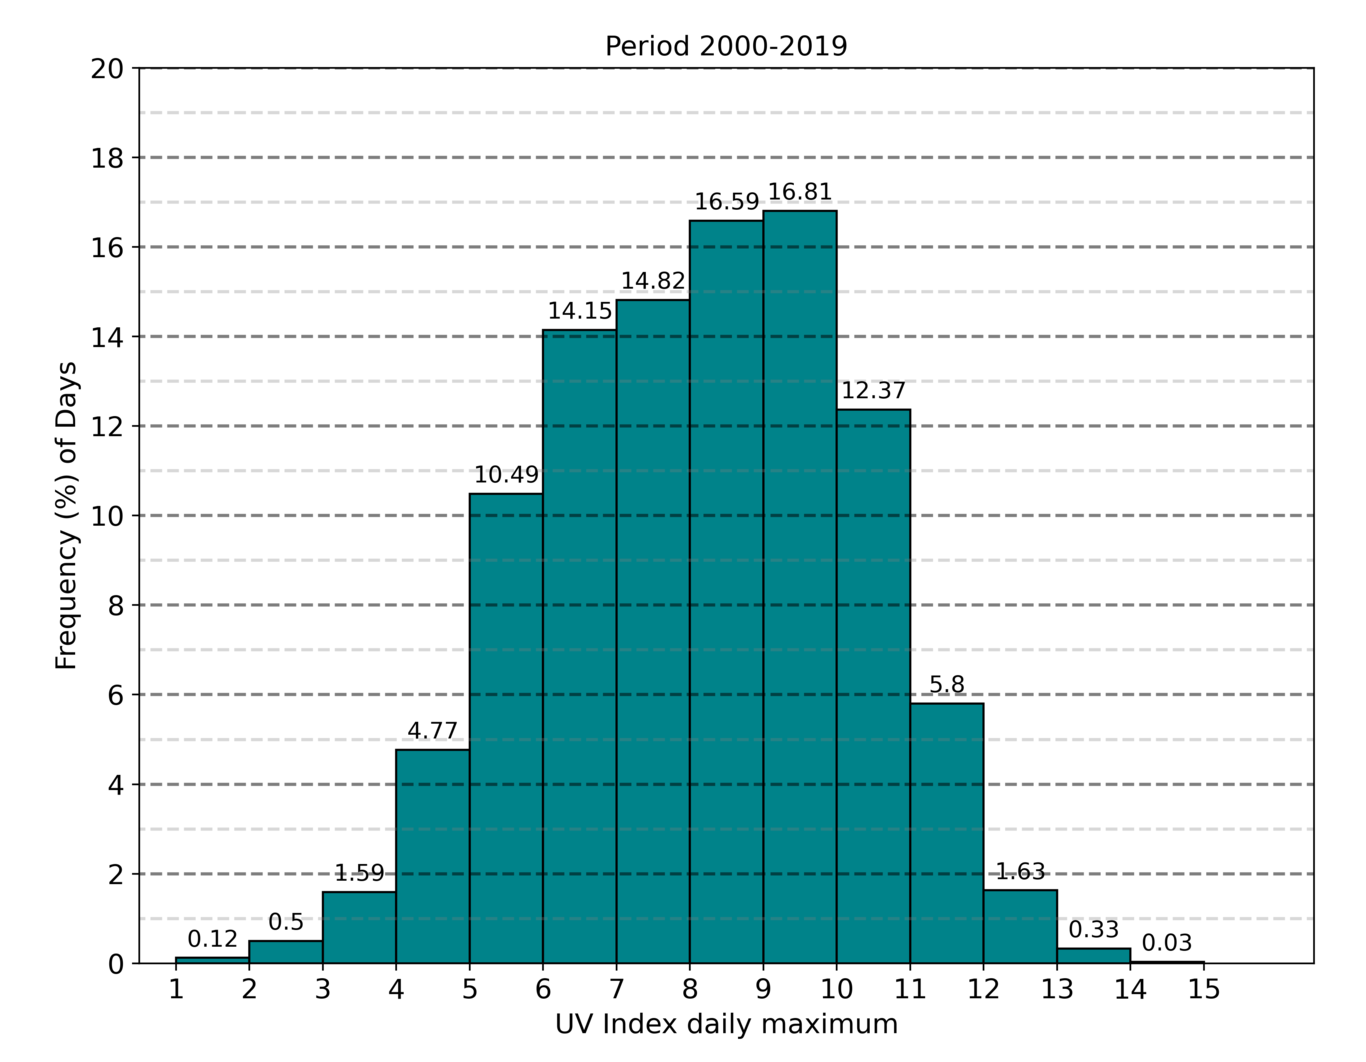
\includegraphics[width=0.49\columnwidth]{figures/HistTotal/HistTotal}
\caption{{Frequency distribution of daily maximum UV Index values in Mexico City
during 2000 -2019.
{\label{461017}}%
}}
\end{center}
\end{figure}

Similar patterns are found when considering the monthly averages
(\(\overline{UVI}_m\)) of daily~\(UVI_{\max}\) as shown in
Figure~{\ref{310112}}. The long-term averages present a
seasonal variation (as in Fig.~{\ref{628947}}),
following approximately the cosine of the noontime solar zenith angle.
Notably, values rarely if ever exceed 12 (as in
Fig.~{\ref{461017}}). Long term trends
in~\(\overline{UVI}_m\) are shown in
Figure~{\ref{185758}}. A clear~upward trend is seen,
with a slope for the linear fit of 0.7\%/year or +1.2 UVI units over the
two decades.\selectlanguage{english}
\begin{figure}[H]
\begin{center}
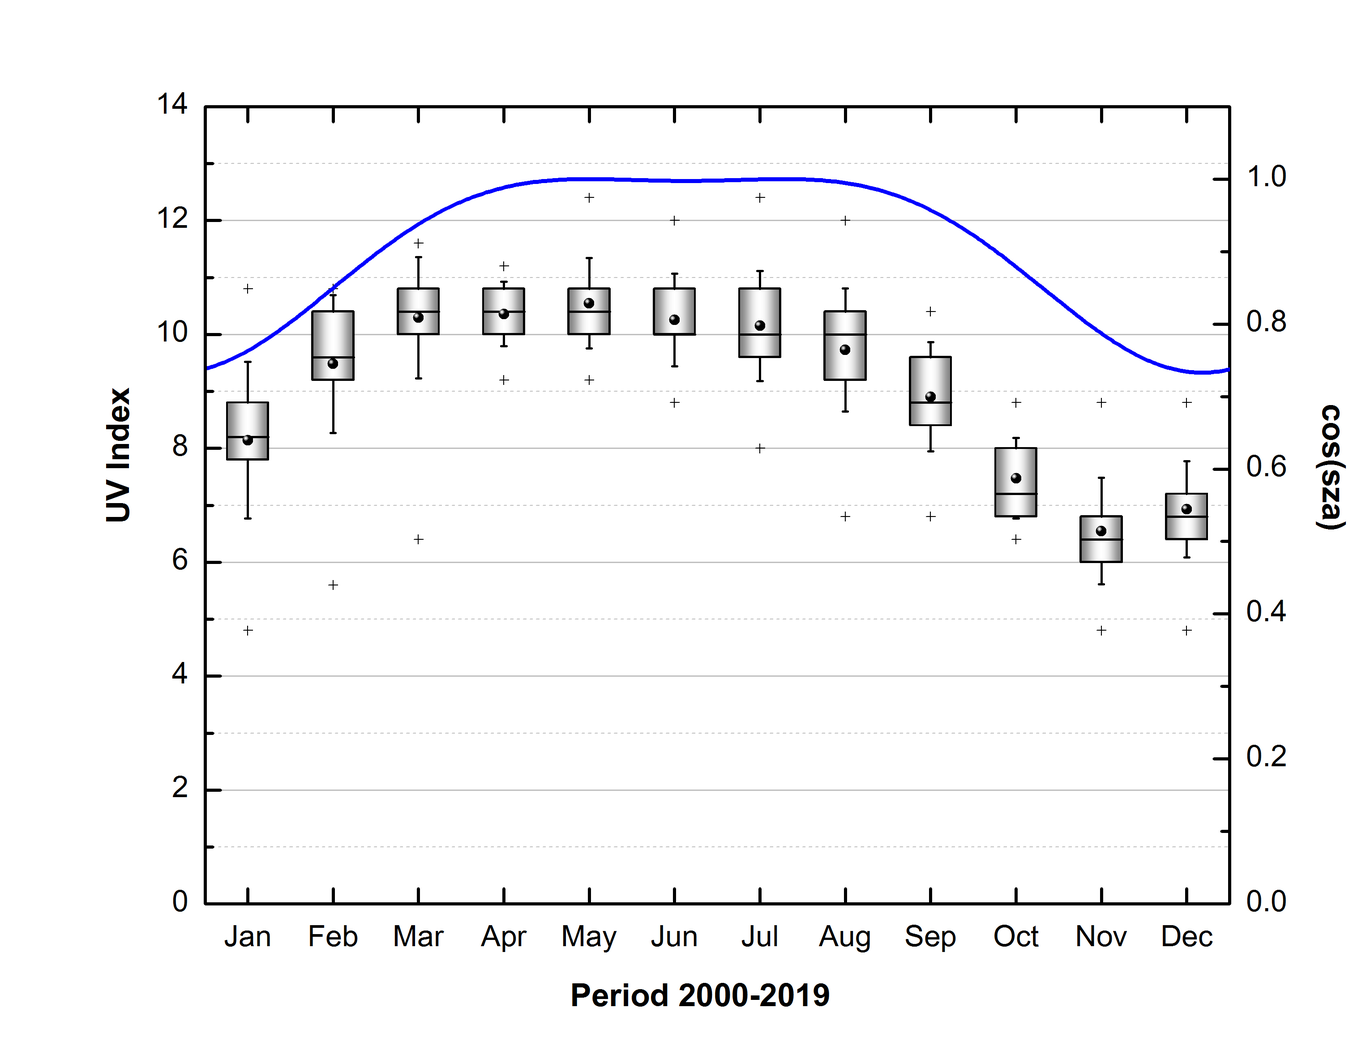
\includegraphics[width=0.70\columnwidth]{figures/Boxplotcos/Boxplotcos}
\caption{{Boxplot of monthly UV Index in MCMA for the period 2000-2019: median
(central bold line), average (black dot), 25\textsuperscript{th} and
75\textsuperscript{th} percentiles (box edges), standard deviation (the
whiskers), the minimum and maximum values (plus sign) and the cosine of
the solar zenith angle at solar noon (blue curve).
{\label{310112}}%
}}
\end{center}
\end{figure}\selectlanguage{english}
\begin{figure}[H]
\begin{center}
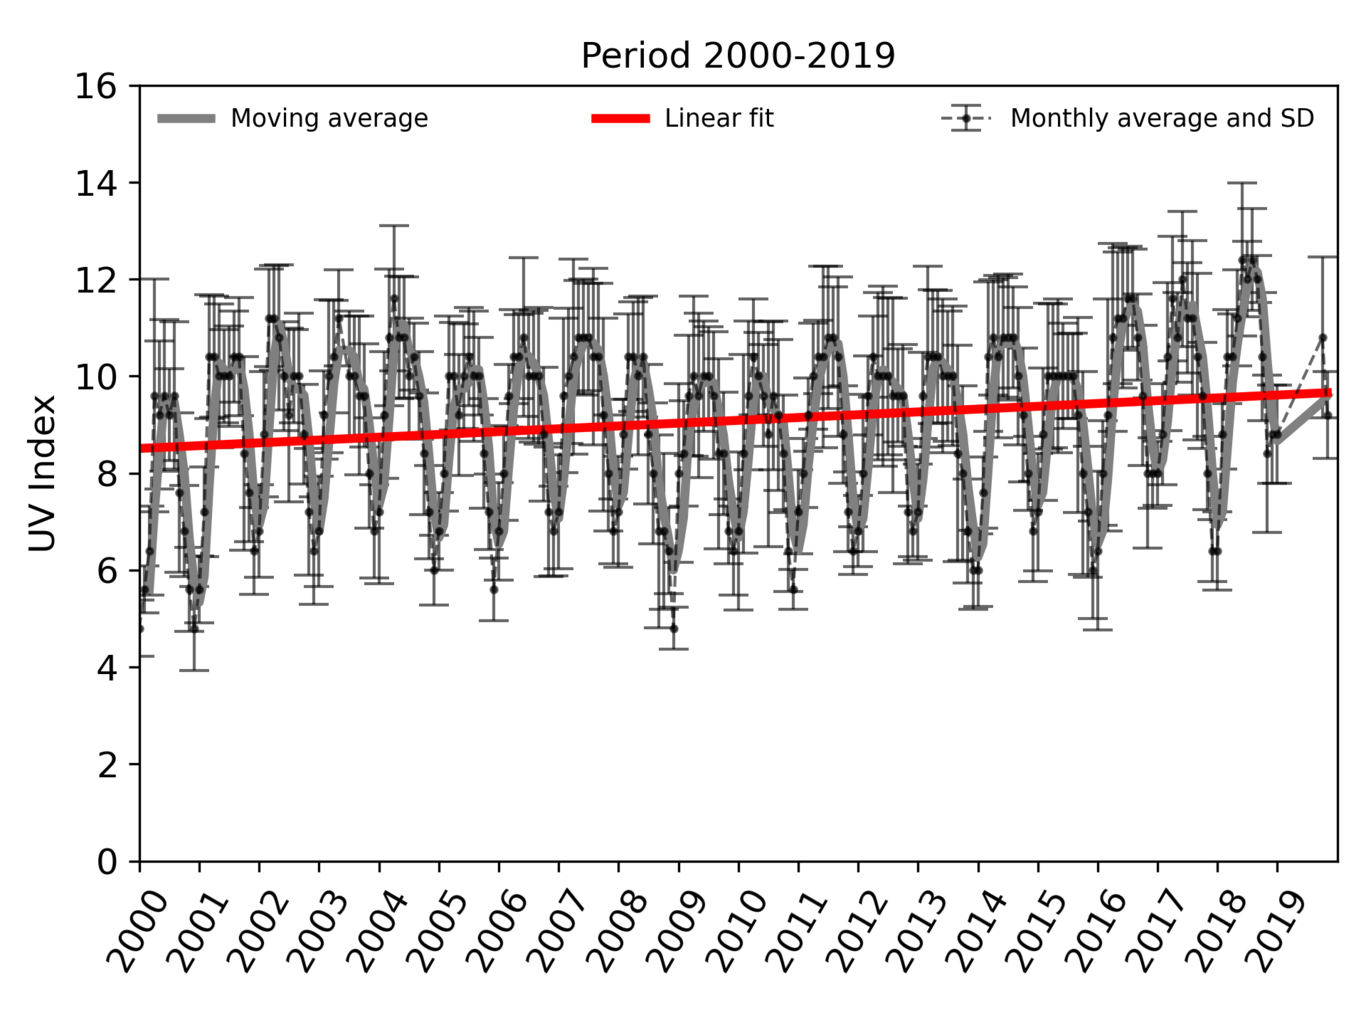
\includegraphics[width=0.70\columnwidth]{figures/CloudDaily/UVyearlyError}
\caption{{Moving average function (gray curve) applied to monthly average UV
Index, standard deviation (black dots and dash line) and linear fit (red
line).
{\label{185758}}%
}}
\end{center}
\end{figure}

The UV Index computed from satellite-based observations
(OMI-Aura/NIVR-FMI-NASA) over the period 2005-2019 is mapped in
Figure~{\ref{485116}}. The satellite-derived UVIs vary
from 8 in winter to 15 in summer, both values being substantially higher
than the ground-based observations (ca. 6 for winter and 11 for summer,
see Fig.~{\ref{310112}}). We hypothesize that this
large difference between satellite-based estimation and ground-based
observation of the UV index is due to the intense air pollution of
Mexico City.~A rather similar behavior was detected in Santiago city,
Chile.~\textsuperscript{\hyperref[csl:46]{46}}\selectlanguage{english}
\begin{figure}[H]
\begin{center}
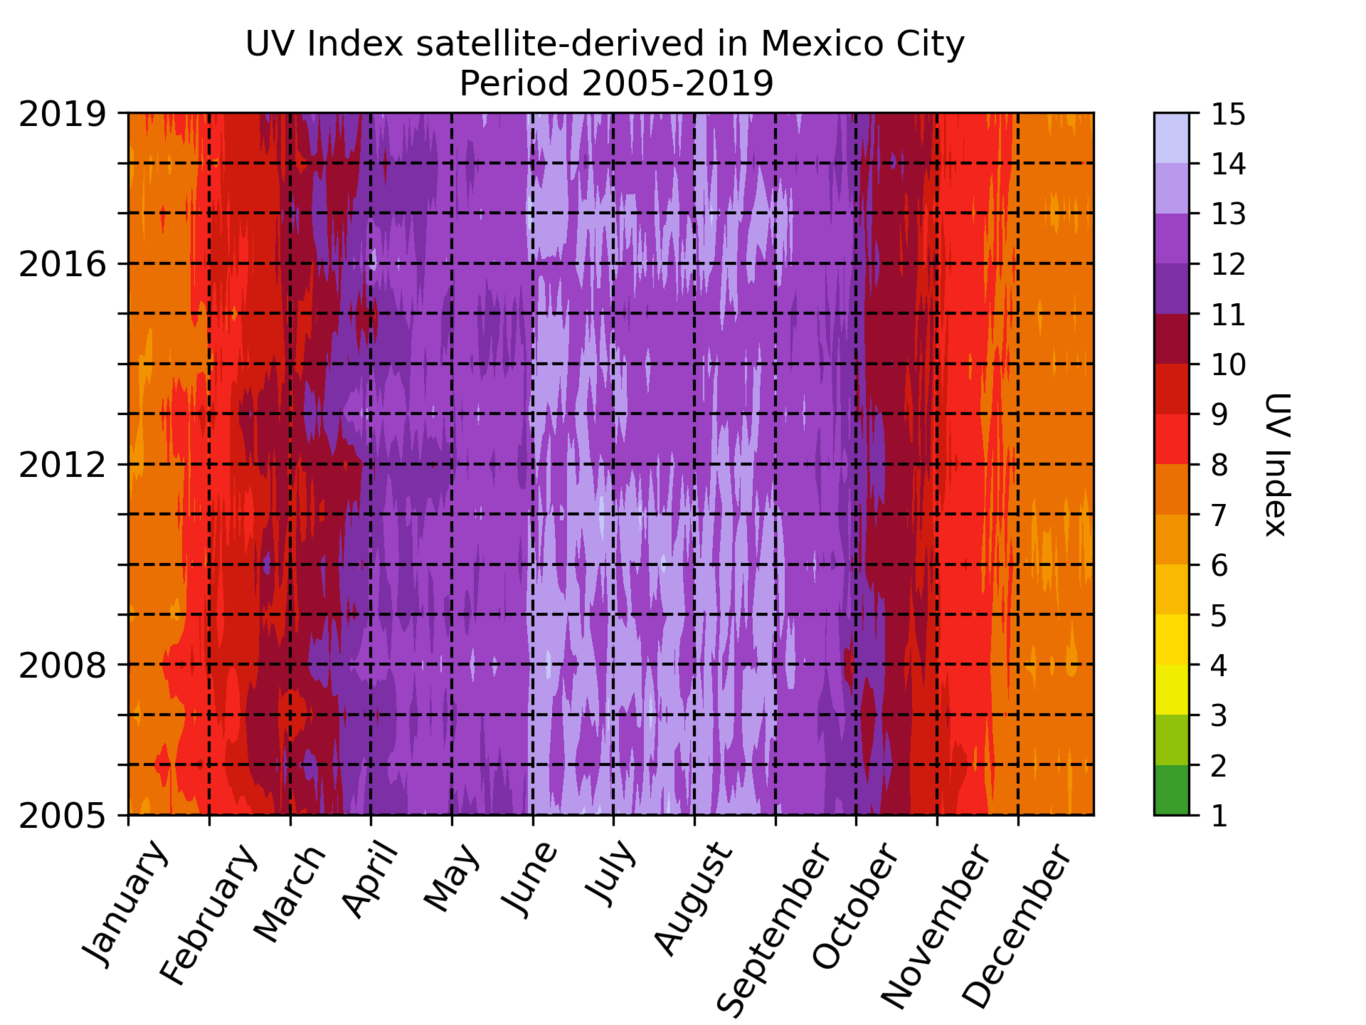
\includegraphics[width=0.70\columnwidth]{figures/UVI-OMI/UVI-OMI}
\caption{{UV Index recorded by OMI-Aura/NIVR-FMI-NASA, from 2005 to 2019.
{\label{485116}}%
}}
\end{center}
\end{figure}

\subsection*{Effect of pollutants on UV
radiation}

{\label{884442}}

Trends and averages in aerosol optical depth AOD\textsubscript{340} and
criteria pollutants PM\textsubscript{10}, CO, NO\textsubscript{2},
O\textsubscript{3~}and SO\textsubscript{2} observed at the SIMAT
stations over 2000-2019, are shown in
Figure~{\ref{829996}} and summarized in
Table~{\ref{table:uvindex}} together with
the~\(UVI_{\max}\). Similar trends have been noted
before~\emph{\textsuperscript{\hyperref[csl:47]{47},\hyperref[csl:48]{48},\hyperref[csl:49]{49}}} and reflect the long-term success of
emission reduction policies and programs.

The observed changes in the concentrations of these air pollutants have
significant implications for surface UV radiation, as can be
demonstrated with the TUV radiative transfer model (see
Table~{\ref{table:TUVmodel}}). The UVI under an ideally
clear atmosphere would reach 15.9 (at noon on 21 June), but pollutant
concentrations in the year 2000 (estimated from
Table~{\ref{table:uvindex}} and
Fig.~{\ref{829996}}) reduce the UVI by nearly 40\%,
down to 9.7. Most of this reduction is due to aerosols in the ABL, with
additional contributions from aerosols in the free troposphere (FT), and
ABL gaseous O\textsubscript{3}, NO\textsubscript{2}, and
SO\textsubscript{2} in order of decreasing importance. The
pollution-related UV reductions in 2019 are less severe, with UVI
increasing by 14\% to 11.1 over the two decades, but still 30\% below
values of ideally clean skies. Thus, the model calculations for clear
skies are in good agreement with the satellite-derived UVI values, and
the model calculations with observed pollutants are in good agreement
with ground-based UVI values, even reflecting their long-term trend.\selectlanguage{english}
\begin{figure}[H]
\begin{center}
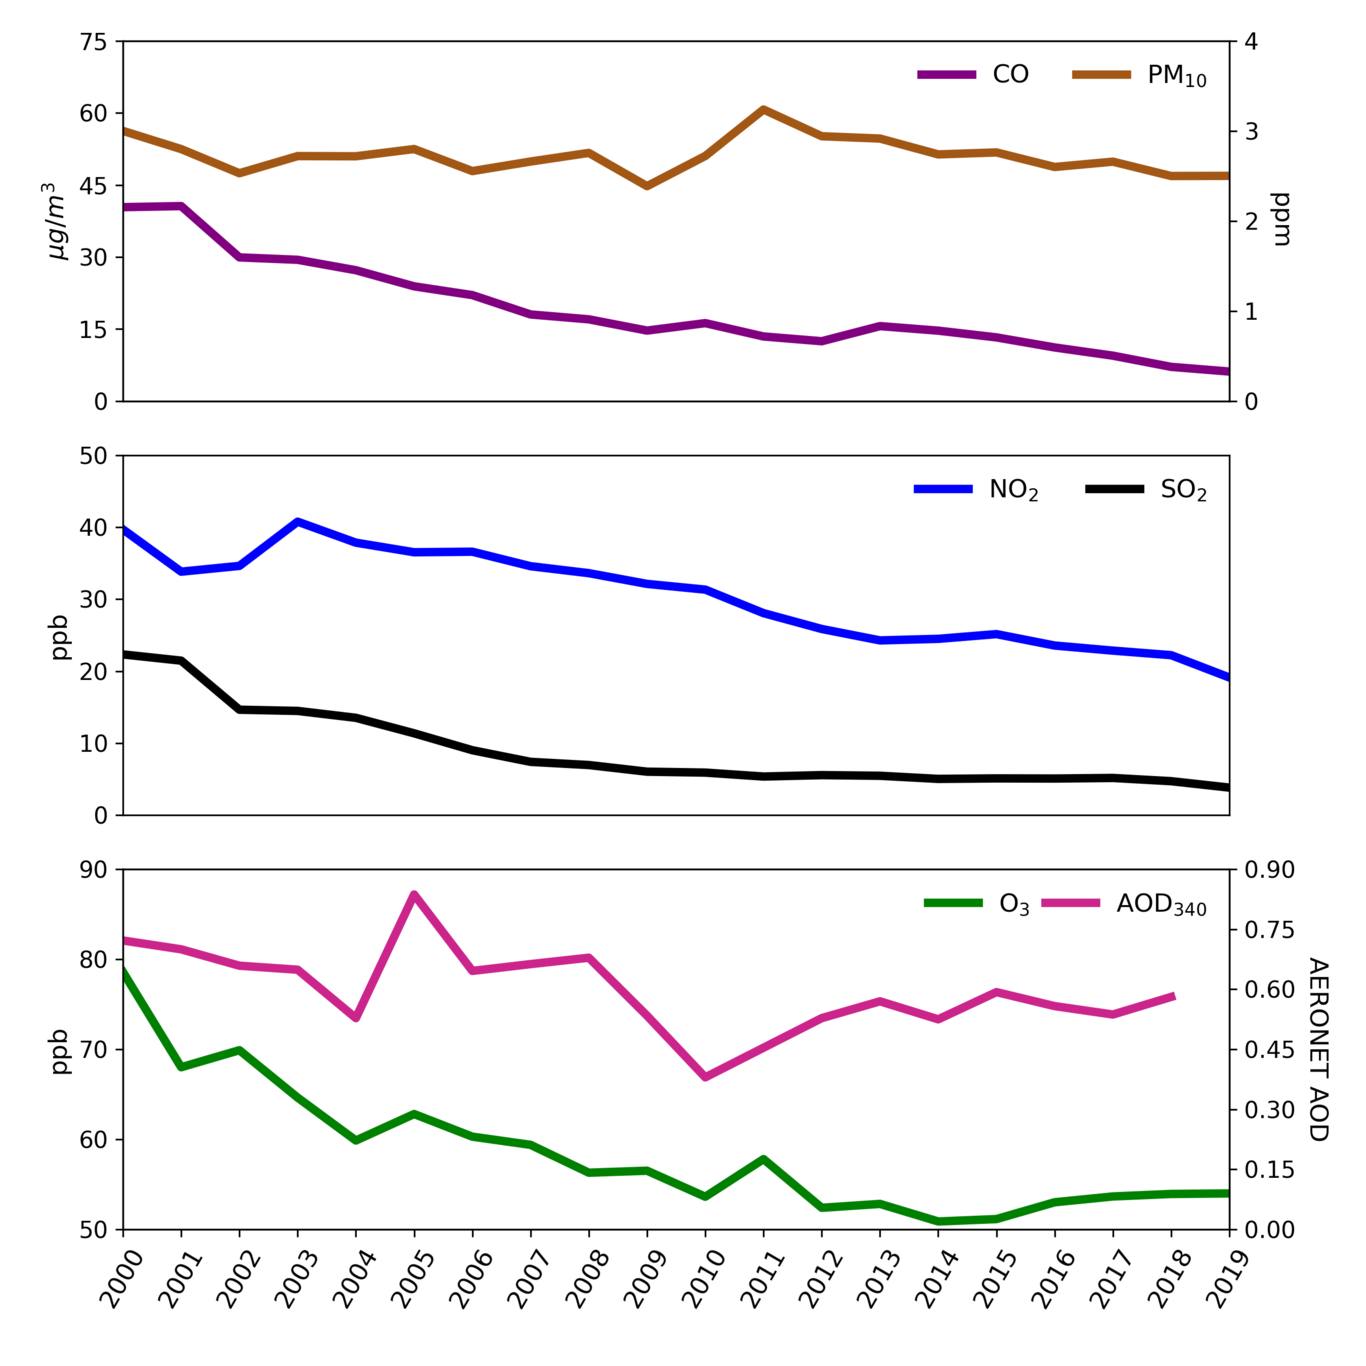
\includegraphics[width=0.63\columnwidth]{figures/contCDMX/contCDMX}
\caption{{Air quality trends in MCMA for the period 2000-2019~ from annual
averages obtained between 11h to 14h CST every day: PM\textsubscript{10}
(brown curve), CO (purple curve), NO\textsubscript{2} (blue curve),
SO\textsubscript{2}(black curve), O\textsubscript{3} (green curve) and
AOD\textsubscript{340} (pink curve).
{\label{829996}}%
}}
\end{center}
\end{figure}\selectlanguage{english}
\begin{table}[H]
\centering
\begin{tabular}{cccc} \hline
Variable &$\frac{\Delta variable}{\Delta t}$ & Avg$_{2000-2019}$ & $\Delta(\%/year)$\\ \hline
UVI &0.06 &9.1 &0.7 \\
PM\textsubscript{10} &-0.12 & 51.1& -0.2\\ 
CO &-0.08 &1.0 &-8.2\\ 
NO\textsubscript{2} &-1.04 & 30.4 &-3.4\\ 
O\textsubscript{3} &-1.05 & 58.5 &-1.8\\ 
AOD\textsubscript{340} &-0.01 &0.6 &-1.6\\
SO\textsubscript{2} & -0.82 &8.9 & -9.2\\
\hline
\end{tabular}
\caption{{{{UV Index and criteria pollutants: slope for the period 2000-2019, averages in units of $\mu g/m^3$(PM$_{10}$), ppm (CO), ppb (SO$_2$, NO$_2$ and O$_3$), dimensionless (UV Index and AOD$_{340}$) and annual percentage change (\%/year).}}}}
\label{table:uvindex}
\end{table}

{Comparable UV reductions, of 30-40\% due to aerosols, were reported by
Panicker et al.}\textsuperscript{\hyperref[csl:11]{11}}{ over Pune, India from April 2004 to
March 2005, with sensitivity coefficients (i.e. change in UVI per unit
change in AOD) similar to those found here in
Table~}{\ref{table:TUVmodel}}{. Over Europe,
ground-based UVI observations for several decades are systematically
lower than those estimated from satellites even after consideration of
climatological aerosol distributions, showing the importance of local
pollution not resolved from space.}\textsuperscript{\hyperref[csl:50]{50}}\selectlanguage{english}
\begin{table}[H]
\centering
\begin{tabular}{lcc} \hline
\textbf{Conditions} & \textbf{UV Index at Noon 21 June} & \textbf{Description} \\ \hline
Clean PBL & 15.9 & \\ \hline
Year 2000 - Aerosols AOD:&\multirow{3}{*}{9.7}& \multirow{3}{5cm}{-6.2 (a 39\% reduction from clean atmosphere)} \\ 0.23 in FT, 0.7 in PBL;\\ O\textsubscript{3}=70, NO\textsubscript{2}=40, SO\textsubscript{2}=10 ppb\\ \hline
Excluding FT aerosols & 10.8 & +1.1 \\\hline
Excluding PBL aerosols & 12.7 & +3.0 \\\hline
Excluding PBL O\textsubscript{3} & 10.4 & +0.7 \\\hline
Excluding PBL NO\textsubscript{2} & 10.1 & +0.4 \\\hline
Excluding PBL SO\textsubscript{2} & 9.9 & +0.2\\\hline
Year 2019 - Aerosol AOD: & \multirow{4}{*}{11.1} & \multirow{4}{5cm}{+1.4 (relative to 2000) a 14\% increase; +4.8 (relative to clean atmosphere) still 30\% reduction from clean atmosphere}\\
0.23 in FT, 0.5 in PBL;\\ O\textsubscript{3}=50, NO\textsubscript{2}=20, SO\textsubscript{2}=1 ppb\\ &&\\\hline
\end{tabular}
\caption{{TUV Model Calculation Illustrating the Effect of Pollutants on the UV Index in Mexico City. The contribution of each pollutant is evaluated by subtraction from the full mixture, rather than individual additions to clean air, to represent more faithfully the interaction between scattering and absorption, e.g. scattering-induced changes in photon path lengths through absorbing gases.}}
\label{table:TUVmodel}
\end{table}

UV reductions by air pollutants are expected to be most severe near the
surface. Thus, such reductions cannot be applied directly to the
photochemical processing that occurs throughout the ABL. If the aerosols
are optically thin and moderately absorbing (as is the case here), the
reduction in vertically averaged UV can be estimated crudely as half of
the reduction seen at the surface (e.g., Castro et
al.~\textsuperscript{\hyperref[csl:44]{44}}, see their Fig. 7). However, scattering
complicates the situation, and a full radiative transfer calculation is
preferable to such crude estimates, with the observed surface UVI used
to anchor the model at the lower boundary.

An issue that is beginning to gain relevance in radiative balance models
is the influence of a group of organic compounds capable of strongly
absorbing in the UV region (brown carbon).\textsuperscript{\hyperref[csl:51]{51}} Some of
these compounds are related with emissions from local and regional
wildfires.\textsuperscript{\hyperref[csl:52]{52}} Mexico City is frequently exposed to
regional fire smoke transport during the dry part of the year (November
to May)\textsuperscript{\hyperref[csl:53]{53}}, that sporadically modify the optical
properties of the aerosols.\textsuperscript{\hyperref[csl:54]{54}} This could partly explain
the relatively minor reductions in PM\textsubscript{10} (see
Fig.~{\ref{829996}}), compared to the larger reductions
of CO, NO\textsubscript{2}, and O\textsubscript{3} that are more
directly related to urban activities, as well as some of the seasonal
asymmetry seen in Fig. {\ref{461017}}. ~

The UVI is specific to wavelengths mainly in the 300-320 nm range, and
so the question remains whether these results can be applied at longer
UV wavelengths, e.g. those important for NO\textsubscript{2} photolysis
(\textless{}420 nm). Absorption by SO\textsubscript{2} and
O\textsubscript{3} vanishes, while absorption by NO\textsubscript{2}
increases and typical aerosols optical depth decrease. These changes can
easily be modeled, but unfortunately far fewer measurements of these
longer wavelengths are available in Mexico City or elsewhere.

\section*{Conclusion}\label{conclusion}

Two decades of observations in Mexico City demonstrate unequivocally
that air pollution reduces UV radiation at the ground. The ground-based
observations are well below estimates derived from satellite-based
observations, and below model calculations do not consider optically
important pollutant aerosols, tropospheric ozone, and to a lesser extent
NO\textsubscript{2} and SO\textsubscript{2}. When typical observed
values of these pollutants are included in a model (e.g. TUV), the
differences between satellite-derived and ground-based measured values
are explained and can be attributed quantitatively to individual
observed pollutants. Long term improvements in air quality, over two
decades, are accompanied by statistically significant increases in the
observed UVI, again in good agreement with the model-predicted changes.
~

The reductions in surface UV radiation with respect to an ideally clear
atmosphere -- by 40\% in 2000 and still 30\% in 2020 -- are large, be it
the context of human UV exposure or air quality mitigation. In urban
areas where ozone production scales proportionally with UV levels and
with volatile organic compound~(VOC) emissions (the VOC-limited regime),
a 20\% increase in average UV means that VOC emissions will need to be
reduced by 20\% to meet the same values, or else successful reductions
in aerosols would lead to unwanted UV-driven increases in
O\textsubscript{3}. Given the importance of the formation of
photochemical secondary compounds in the degradation of the air quality,
it is advisable to extend a study of the impacts in the changes of
actinic flux.~The efforts that Mexico City has made to improve air
quality have achieved positive results in the levels of most air
pollutants. Nevertheless, ironically they caused an increase in UV
radiation that reaches the surface, which could have consequences on
human health. For human exposure, a 30\% increase in UV-induced skin
cancer and cataract would constitute a non-negligible public health
issue and require a reassessment of preventive behaviors. ~

A limitation of the present work is our focus on daily maximum values,
which largely exclude cloud cover. Absorption within clouds can be
enhanced by the long path lengths of multiply scattered photons (e.g.,
Mayer et al.\textsuperscript{\hyperref[csl:55]{55}}), so that accurate quantification of UV
effects of clouds in polluted environments remains a significant
challenge and interesting opportunity for future work.~

\section*{Acknowledgements}\label{acknowledgements}

We wish to acknowledge the staff of SIMAT, from the Secretariat of
Environment, for the data and the continuous assistance during the
realization of this project. Adriana Ipi\selectlanguage{ngerman}ña would like to extend her
thanks to\textbf{~}Dirección General de Personal Académico, Universidad
Nacional Autónoma~de México (DGAPA-UNAM) for the postdoctoral fellowship
at Centro de Ciencias~de la Atmósfera of the UNAM.~Rubén D Piacentini
wishes to thank CONICET and National University of Rosario, Argentina,
for their partial support to the present work.~The National Center for
Atmospheric Research is sponsored by the National Science Foundation.

\selectlanguage{english}
\FloatBarrier
\section*{References}\sloppy
\phantomsection
\label{csl:1}(1) Taylor, H. R.; West, S. K.; Rosenthal, F. S.; Mu{\~{n}}oz, B.; Newland, H. S.; Abbey, H.; Emmett, E. A. {Effect of Ultraviolet Radiation on Cataract Formation}. \textit{New England Journal of Medicine} \textbf{1988}, \textit{319} (22), 1429–1433. \url{https://doi.org/10.1056/nejm198812013192201.}

\phantomsection
\label{csl:2}(2) Varotsos, C.; Feretis, E. {Health Effects on Human Eye Resulting from the Increased Ambient Solar Ultraviolet Radiation}. \textit{Toxicological {\&} Environmental Chemistry} \textbf{1997}, \textit{61} (1-4), 43–68. \url{https://doi.org/10.1080/02772249709358473.}

\phantomsection
\label{csl:3}(3) Lucas, R. M.; Yazar, S.; Young, A. R.; Norval, M.; de-Gruijl, F. R.; Takizawa, Y.; Rhodes, L. E.; Sinclair, C. A.; Neale, R. E. {Human Health in Relation to Exposure to Solar Ultraviolet Radiation under Changing Stratospheric Ozone and Climate}. \textit{Photochemical {\&} Photobiological Sciences} \textbf{2019}, \textit{18} (3), 641–680. \url{https://doi.org/10.1039/c8pp90060d.}

\phantomsection
\label{csl:4}(4) Leighton, P. A. {Physical Chemistry}. In \textit{Photochemistry of Air Pollution}; Elsevier, 1961; pp v--vi. \url{https://doi.org/10.1016/b978-0-12-442250-6.50004-3.}

\phantomsection
\label{csl:5}(5) Seinfeld, J. H.; Pandis, S. N.; Noone, K. {Atmospheric Chemistry and Physics: From Air Pollution to Climate Change}. \textit{Physics Today} \textbf{1998}, \textit{51} (10), 88–90. \url{https://doi.org/10.1063/1.882420.}

\phantomsection
\label{csl:6}(6) Finlayson-Pitts, B. J.; Pitts, J. N. {Theory, Experiments, and Applications}. In \textit{Chemistry of the Upper and Lower Atmosphere}; Elsevier, 2000; pp xvii--xviii. \url{https://doi.org/10.1016/b978-012257060-5/50000-9.}

\phantomsection
\label{csl:7}(7) Liu, S. C.; McKeen, S. A.; Madronich, S. {Effect of Anthropogenic Aerosols on Biologically Active Ultraviolet Radiation}. \textit{Geophysical Research Letters} \textbf{1991}, \textit{18} (12), 2265–2268. \url{https://doi.org/10.1029/91gl02773.}

\phantomsection
\label{csl:8}(8) Sabziparvar, A. A.; Forster, P. M. F.; Shine, K. P. {Changes in Ultraviolet Radiation Due to Stratospheric and Tropospheric Ozone Changes since Preindustrial Times}. \textit{Journal of Geophysical Research: Atmospheres} \textbf{1998}, \textit{103} (D20), 26107–26113. \url{https://doi.org/10.1029/98jd02277.}

\phantomsection
\label{csl:9}(9) Madronich, S.; Wagner, M.; Groth, P. {Influence of Tropospheric Ozone Control on Exposure to Ultraviolet Radiation at the Surface}. \textit{Environmental Science {\&} Technology} \textbf{2011}, \textit{45} (16), 6919–6923. \url{https://doi.org/10.1021/es200701q.}

\phantomsection
\label{csl:10}(10) McKenzie, R. L.; Weinreis, C.; Johnston, P. V.; Liley, B.; Shiona, H.; Kotkamp, M.; Smale, D.; Takegawa, N.; Kondo, Y. {Effects of Urban Pollution on {UV} Spectral Irradiances}. \textit{Atmospheric Chemistry and Physics} \textbf{2008}, \textit{8} (18), 5683–5697. \url{https://doi.org/10.5194/acp-8-5683-2008.}

\phantomsection
\label{csl:11}(11) Panicker, A. S.; Pandithurai, G.; Takamura, T.; Pinker, R. T. {Aerosol Effects in the {UV}-B Spectral Region over Pune an Urban Site in India}. \textit{Geophysical Research Letters} \textbf{2009}, \textit{36} (10). \url{https://doi.org/10.1029/2009gl037632.}

\phantomsection
\label{csl:12}(12) Palancar, G. G.; Lefer, B. L.; Hall, S. R.; Shaw, W. J.; Corr, C. A.; Herndon, S. C.; Slusser, J. R.; Madronich, S. {Effect of Aerosols and NO$_{2}$ Concentration on Ultraviolet Actinic Flux near Mexico City during MILAGRO: Measurements and Model Calculations}. \textit{Atmospheric Chemistry and Physics} \textbf{2013}, \textit{13} (2), 1011–1022. \url{https://doi.org/10.5194/acp-13-1011-2013.}

\phantomsection
\label{csl:13}(13) Bais, A. F.; McKenzie, R. L.; Bernhard, G.; Aucamp, P. J.; Ilyas, M.; Madronich, S.; Tourpali, K. {Ozone Depletion and Climate Change: Impacts on {UV} Radiation}. \textit{Photochemical {\&} Photobiological Sciences} \textbf{2015}, \textit{14} (1), 19–52. \url{https://doi.org/10.1039/c4pp90032d.}

\phantomsection
\label{csl:14}(14) Hollaway, M.; Wild, O.; Yang, T.; Sun, Y.; Xu, W.; Xie, C.; Whalley, L.; Slater, E.; Heard, D.; Liu, D. {Photochemical Impacts of Haze Pollution in an Urban Environment}. \textit{Atmospheric Chemistry and Physics} \textbf{2019}, \textit{19} (15), 9699–9714. \url{https://doi.org/10.5194/acp-19-9699-2019.}

\phantomsection
\label{csl:15}(15) Li, K.; Jacob, D. J.; Liao, H.; Shen, L.; Zhang, Q.; Bates, K. H. {Anthropogenic Drivers of 2013-2017 Trends in Summer Surface Ozone in China}. \textit{Proceedings of the National Academy of Sciences} \textbf{2018}, \textit{116} (2), 422–427. \url{https://doi.org/10.1073/pnas.1812168116.}

\phantomsection
\label{csl:16}(16) Wang, Y.; Gao, W.; Wang, S.; Song, T.; Gong, Z.; Ji, D.; Wang, L.; Liu, Z.; Tang, G.; Huo, Y.; et al. {Contrasting Trends of {PM}2.5 and Surface-Ozone Concentrations in China from 2013 to 2017}. \textit{National Science Review} \textbf{2020}, \textit{7} (8), 1331–1339. \url{https://doi.org/10.1093/nsr/nwaa032.}

\phantomsection
\label{csl:17}(17) Wang, W.; Li, X.; Shao, M.; Hu, M.; Zeng, L.; Wu, Y.; Tan, T. {The Impact of Aerosols on Photolysis Frequencies and Ozone Production in  Beijing during the 4-Year Period 2012-2015}. \textit{Atmospheric Chemistry and Physics} \textbf{2019}, \textit{19} (14), 9413–9429. \url{https://doi.org/10.5194/acp-19-9413-2019.}

\phantomsection
\label{csl:18}(18) Gao, J.; Li, Y.; Zhu, B.; Hu, B.; Wang, L.; Bao, F. {What Have We Missed When Studying the Impact of Aerosols on Surface Ozone via Changing Photolysis Rates?}. \textbf{2020}. \url{https://doi.org/10.5194/acp-2020-140.}

\phantomsection
\label{csl:19}(19) Ma, X.; Huang, J.; Zhao, T.; Liu, C.; Zhao, K.; Xing, J.; Xiao, W. {Rapid Increase in Summer Surface Ozone over the North China Plain during 2013-2019: a Side Effect of Particulate Matters Reduction Control?}. \textbf{2020}. \url{https://doi.org/10.5194/acp-2020-385.}

\phantomsection
\label{csl:20}(20) Bauwens, M.; Compernolle, S.; Stavrakou, T.; Müller, J.-F.; Gent, J.; Eskes, H.; Levelt, P. F.; A, R.; Veefkind, J. P.; Vlietinck, J.; et al. {Impact of Coronavirus Outbreak on NO2 Pollution Assessed Using TROPOMI and OMI Observations}. \textbf{2020}, \textit{47} (11). \url{https://doi.org/10.1029/2020gl087978.}

\phantomsection
\label{csl:21}(21) Venter, Z. S.; Aunan, K.; Chowdhury, S.; Lelieveld, J. {{COVID}-19 Lockdowns Cause Global Air Pollution Declines}. \textit{Proceedings of the National Academy of Sciences} \textbf{2020}, \textit{117} (32), 18984–18990. \url{https://doi.org/10.1073/pnas.2006853117.}

\phantomsection
\label{csl:22}(22) Shi, X.; Brasseur, G. P. {The Response in Air Quality to the Reduction of Chinese Economic Activities During the {COVID}-19 Outbreak}. \textit{Geophysical Research Letters} \textbf{2020}, \textit{47} (11). \url{https://doi.org/10.1029/2020gl088070.}

\phantomsection
\label{csl:23}(23) Le, T.; Wang, Y.; Liu, L.; Yang, J.; Yung, Y. L.; Li, G.; Seinfeld, J. H. {Unexpected Air Pollution with Marked Emission Reductions during the {COVID}-19 Outbreak in China}. \textit{Science} \textbf{2020}, \textit{369} (6504), 702–706. \url{https://doi.org/10.1126/science.abb7431.}

\phantomsection
\label{csl:24}(24) \textit{{Red Automática De Monitoreo Atmosférico (RAMA)}}; \url{http://www.aire.cdmx.gob.mx/descargas/datos/excel/RAMAxls.pdf.}

\phantomsection
\label{csl:25}(25) Doran, J. C.; Abbott, S.; Archuleta, J.; Bian, X.; Chow, J.; Coulter, R. L.; Wekker, S. F. J. de; Edgerton, S.; Elliott, S.; Fernandez, A.; et al. {The IMADA-AVER Boundary Layer Experiment in the Mexico City Area}. \textit{Bulletin of the American Meteorological Society} \textbf{1998}, \textit{79} (11), 2497–2508. \url{https://doi.org/10.1175/1520-0477(1998)079<2497:TIABLE>2.0.CO;2.}

\phantomsection
\label{csl:26}(26) Molina, L. T.; Kolb, C. E.; Foy, B. de; Lamb, B. K.; Brune, W. H.; Jimenez, J. L.; Ramos-Villegas, R.; Sarmiento, J.; Paramo-Figueroa, V. H.; Cardenas, B.; et al. {Air Quality in North America's Most Populous City - Overview of the {MCMA}-2003 Campaign}. \textit{Atmospheric Chemistry and Physics} \textbf{2007}, \textit{7} (10), 2447–2473. \url{https://doi.org/10.5194/acp-7-2447-2007.}

\phantomsection
\label{csl:27}(27) Molina, L. T.; Madronich, S.; Gaffney, J. S.; Apel, E.; Foy, B. de; Fast, J.; Ferrare, R.; Herndon, S.; Jimenez, J. L.; Lamb, B.; et al. {An Overview of the {MILAGRO} 2006 Campaign: Mexico City Emissions and Their Transport and Transformation}. \textit{Atmospheric Chemistry and Physics} \textbf{2010}, \textit{10} (18), 8697–8760. \url{https://doi.org/10.5194/acp-10-8697-2010.}

\phantomsection
\label{csl:28}(28) Jazcilevich, A. D.; Garc{\'{\i}}a, A. R.; Caetano, E. {Locally Induced Surface Air Confluence by Complex Terrain and Its Effects on Air Pollution in the Valley of Mexico}. \textit{Atmospheric Environment} \textbf{2005}, \textit{39} (30), 5481–5489. \url{https://doi.org/10.1016/j.atmosenv.2005.05.046.}

\phantomsection
\label{csl:29}(29) Tie, X.; Madronich, S.; Li, G. H.; Ying, Z.; Zhang, R.; Garcia, A. R.; Lee-Taylor, J.; Liu, Y. {Characterizations of Chemical Oxidants in Mexico City: A Regional Chemical Dynamical Model ({WRF}-Chem) Study}. \textit{Atmospheric Environment} \textbf{2007}, \textit{41} (9), 1989–2008. \url{https://doi.org/10.1016/j.atmosenv.2006.10.053.}

\phantomsection
\label{csl:30}(30) Zhang, Y.; Dubey, M. K.; Olsen, S. C.; Zheng, J.; Zhang, R. {Comparisons of {WRF}/Chem Simulations in Mexico City with Ground-Based {RAMA} Measurements during the 2006-{MILAGRO}}. \textit{Atmospheric Chemistry and Physics} \textbf{2009}, \textit{9} (11), 3777–3798. \url{https://doi.org/10.5194/acp-9-3777-2009.}

\phantomsection
\label{csl:31}(31) Zavala, M.; Brune, W. H.; Velasco, E.; Retama, A.; Cruz-Alavez, L. A.; Molina, L. T. {Changes in Ozone Production and {VOC} Reactivity in the Atmosphere of the Mexico City Metropolitan Area}. \textit{Atmospheric Environment} \textbf{2020}, \textit{238}, 117747. \url{https://doi.org/10.1016/j.atmosenv.2020.117747.}

\phantomsection
\label{csl:32}(32) \textit{{Secretaría Del Medio Ambiente (SEDEMA)}}; \url{https://www.sedema.cdmx.gob.mx/.}

\phantomsection
\label{csl:33}(33) WHO. \textit{{Global Solar UV Index: A Practical Guide}}; 2002.

\phantomsection
\label{csl:34}(34) Webb, A. R.; Slaper, H.; Koepke, P.; Schmalwieser, A. W. {Know Your Standard: Clarifying the {CIE} Erythema Action Spectrum}. \textit{Photochemistry and Photobiology} \textbf{2011}, \textit{87} (2), 483–486. \url{https://doi.org/10.1111/j.1751-1097.2010.00871.x.}

\phantomsection
\label{csl:35}(35) Whiteman, C. D.; Zhong, S.; Bian, X.; Fast, J. D.; Doran, J. C. {Boundary Layer Evolution and Regional-Scale Diurnal Circulations over the and Mexican Plateau}. \textit{Journal of Geophysical Research: Atmospheres} \textbf{2000}, \textit{105} (D8), 10081–10102. \url{https://doi.org/10.1029/2000jd900039.}

\phantomsection
\label{csl:36}(36) Fast, J. D.; Foy, B. de; Rosas, F. A.; Caetano, E.; Carmichael, G.; Emmons, L.; McKenna, D.; Mena, M.; Skamarock, W.; Tie, X.; et al. {A Meteorological Overview of the {MILAGRO} Field Campaigns}. \textit{Atmospheric Chemistry and Physics} \textbf{2007}, \textit{7} (9), 2233–2257. \url{https://doi.org/10.5194/acp-7-2233-2007.}

\phantomsection
\label{csl:37}(37) \textit{{Sistema De Monitoreo Atmosférico (SIMAT)}}; www.aire.cdmx.gob.mx.

\phantomsection
\label{csl:38}(38) Holben, B. N.; Eck, T. F.; Slutsker, I.; Tanr{\'{e}}, D.; Buis, J. P.; Setzer, A.; Vermote, E.; Reagan, J. A.; Kaufman, Y. J.; Nakajima, T.; et al. {{AERONET}'A Federated Instrument Network and Data Archive for Aerosol Characterization}. \textit{Remote Sensing of Environment} \textbf{1998}, \textit{66} (1), 1–16. \url{https://doi.org/10.1016/s0034-4257(98)00031-5.}

\phantomsection
\label{csl:39}(39) \textit{{NASA EOS/Aura Validation Data Center (AVDC) - Correlative Data, Field of View Predictions, Data Subsets, GEOMS, DCIO}}; \url{https://avdc.gsfc.nasa.gov/pub/most_popular/overpass/OMI/.}

\phantomsection
\label{csl:40}(40) Madronich, S. {Intercomparison of {NO}2 Photodissociation and U.V. Radiometer Measurements}. \textit{Atmospheric Environment} \textbf{1987}, \textit{21} (3), 569–578. \url{https://doi.org/10.1016/0004-6981(87)90039-4.}

\phantomsection
\label{csl:41}(41) Shaw, W. J.; Pekour, M. S.; Coulter, R. L.; Martin, T. J.; Walters, J. T. {The Daytime Mixing Layer Observed by Radiosonde Profiler, and Lidar during {MILAGRO}}. \textit{Atmospheric Chemistry and Physics Discussions} \textbf{2007}, \textit{7} (5), 15025–15065. \url{https://doi.org/10.5194/acpd-7-15025-2007.}

\phantomsection
\label{csl:42}(42) Elterman, L. \textit{{An Atlas of Aerosol Attenuation and Extinction Profiles for the Troposphere and Stratosphere}}; Defense Technical Information Center, 1966. \url{https://doi.org/10.21236/ad0649778.}

\phantomsection
\label{csl:43}(43) Corr, C. A.; Krotkov, N.; Madronich, S.; Slusser, J. R.; Holben, B.; Gao, W.; Flynn, J.; Lefer, B.; Kreidenweis, S. M. {Retrieval of Aerosol Single Scattering Albedo at Ultraviolet Wavelengths at the T1 Site during {MILAGRO}}. \textit{Atmospheric Chemistry and Physics} \textbf{2009}, \textit{9} (15), 5813–5827. \url{https://doi.org/10.5194/acp-9-5813-2009.}

\phantomsection
\label{csl:44}(44) Castro, T.; Madronich, S.; Rivale, S.; Muhlia, A.; Mar, B. {The Influence of Aerosols on Photochemical Smog in Mexico City}. \textit{Atmospheric Environment} \textbf{2001}, \textit{35} (10), 1765–1772. \url{https://doi.org/10.1016/s1352-2310(00)00449-0.}

\phantomsection
\label{csl:45}(45) SEDEMA. \textit{{Calidad Del Aire En La Ciudad De México, Informe 2017}}; Secretaría del Medio Ambiente, Gobierno de la Ciudad de México, México, 2018a.

\phantomsection
\label{csl:46}(46) Cabrera, S.; Ipi{\~{n}}a, A.; Damiani, A.; Cordero, R. R.; Piacentini, R. D. {{UV} Index Values and Trends in Santiago Chile (33.5$\circ$S) Based on Ground and Satellite Data}. \textit{Journal of Photochemistry and Photobiology B: Biology} \textbf{2012}, \textit{115}, 73–84. \url{https://doi.org/10.1016/j.jphotobiol.2012.06.013.}

\phantomsection
\label{csl:47}(47) Parrish, D. D.; Singh, H. B.; Molina, L.; Madronich, S. {Air Quality Progress in North American Megacities: A Review}. \textit{Atmospheric Environment} \textbf{2011}, \textit{45} (39), 7015–7025. \url{https://doi.org/10.1016/j.atmosenv.2011.09.039.}

\phantomsection
\label{csl:48}(48) \textit{{Informe Anual Calidad Del Aire 2017}}; \url{http://www.aire.cdmx.gob.mx/descargas/publicaciones/flippingbook/informe_anual_calidad_aire_2017/mobile/#p=1.}

\phantomsection
\label{csl:49}(49) Molina; Velasco; Retama; Zavala. {Experience from Integrated Air Quality Management in the Mexico City Metropolitan Area and Singapore}. \textit{Atmosphere} \textbf{2019}, \textit{10} (9), 512. \url{https://doi.org/10.3390/atmos10090512.}

\phantomsection
\label{csl:50}(50) Vitt, R.; Laschewski, G.; Bais, A.; Di{\'{e}}moz, H.; Fountoulakis, I.; Siani, A.-M.; Matzarakis, A. {{UV}-Index Climatology for Europe Based on Satellite Data}. \textit{Atmosphere} \textbf{2020}, \textit{11} (7), 727. \url{https://doi.org/10.3390/atmos11070727.}

\phantomsection
\label{csl:51}(51) Laskin, A.; Laskin, J.; Nizkorodov, S. A. {Chemistry of Atmospheric Brown Carbon}. \textit{Chemical Reviews} \textbf{2015}, \textit{115} (10), 4335–4382. \url{https://doi.org/10.1021/cr5006167.}

\phantomsection
\label{csl:52}(52) Gadhavi, H.; Jayaraman, A. {Absorbing Aerosols: Contribution of Biomass Burning and Implications for Radiative Forcing}. \textit{Annales Geophysicae} \textbf{2010}, \textit{28} (1), 103–111. \url{https://doi.org/10.5194/angeo-28-103-2010.}

\phantomsection
\label{csl:53}(53) Rios, B.; Raga, G. B. {Smoke Emissions from Agricultural Fires in Mexico and Central America}. \textit{Journal of Applied Remote Sensing} \textbf{2019}, \textit{13} (03), 1. \url{https://doi.org/10.1117/1.jrs.13.036509.}

\phantomsection
\label{csl:54}(54) Barnard, J. C.; Volkamer, R.; Kassianov, E. I. {Estimation of the Mass Absorption Cross Section of the Organic Carbon Component of Aerosols in the Mexico City Metropolitan Area}. \textit{Atmospheric Chemistry and Physics} \textbf{2008}, \textit{8} (22), 6665–6679. \url{https://doi.org/10.5194/acp-8-6665-2008.}

\phantomsection
\label{csl:55}(55) Mayer, B.; Kylling, A.; Madronich, S.; Seckmeyer, G. {Enhanced Absorption of {UV} Radiation Due to Multiple Scattering in Clouds: Experimental Evidence and Theoretical Explanation}. \textit{Journal of Geophysical Research: Atmospheres} \textbf{1998}, \textit{103} (D23), 31241–31254. \url{https://doi.org/10.1029/98jd02676.}
\end{document}

